\documentclass{article}
% --- Packages (formatting only; wording unchanged) ---
\usepackage[margin=1in]{geometry} % 1 inch margins all around
\usepackage{graphicx,xcolor}
\usepackage{booktabs}
\usepackage{amsmath}
\usepackage{float}      % for [H] exact placement
\usepackage{placeins}   % for \FloatBarrier
\usepackage{caption}
\captionsetup{justification=Centering, skip=0.5\baselineskip}
\usepackage{graphicx} % Required for inserting images
\usepackage[numbers, square]{natbib}
\usepackage{enumitem}

\title{\vspace{-2cm}MAT292 Final Project: TITLE}
\author{Group 11: Arthur Chen - Jerry Jiang - Ben Lian}
\date{October 3, 2025}

\begin{document}

\maketitle

\section{Motivation and Objectives}
``The Video Game Industry (VGI) is a highly innovative and rapidly growing sector [...] with significant economic and social implications. [Yet] the literature remains fragmented and lacks a coherent framework for understanding its complex nature and underlying dynamics." \cite{GOH2023100100} We find that predicting the population of gamers over time can apply our research on the interplay between technological advances, affordability, accessibility, and market saturation.\\

\noindent 
Our project examines PC gamers, who represent a dominant segment influenced by the affordability of commercial hardware, accessibility of internet infrastructure, and emerging technologies in the market (e.g., VR and cloud gaming). Our goal is to develop a differential equation–based model, primarily combining logistic growth and Bass diffusion, to predict the PC gamer population over time, validate and verify it with available adoption data, and study scenario-based technological shocks (e.g., disruptions from VR).

\section{Mathematical and Computational Background}
Our project uses mathematical concepts from MAT292 to model our analysis of the relationship between PC video game players and tech growth. In our elementary stage, we intend to apply Ordinary Differential Equations (ODE) modelling, focusing on models of logistic growth, Bass adoption/diffusion, and possibly compartmental epidemic models. Machine learning (ML) provides contextual background on the adoption dynamics of networks, accounting for the network of social connections. 

\subsection{Logistic Growth Model with Optional Threshold}
Referring to Lecture 07 (Murdock), the logistic equation with carrying capacity is applicable: 

\begin{equation}
    \frac{dP}{dt} = rP \left(1 - \frac{P}{K}\right), 
    \qquad \frac{dP}{dt} = rP \left(1 - \frac{P}{K}\right) \left(1 - \frac{P}{T}\right)
\end{equation}

\noindent $P$ is the gamer population, $r$ is the growth rate, and $K$ is the carrying capacity (maximum sustainable gamers given affordability and infrastructure). Optionally, $T$ is the population threshold necessary for the game to be sustainable under the Allee effect \cite{9b04f3dc-918b-391a-9a53-ddc05d360c66}.  

\subsection{Bass Adoption/Diffusion Model}
The growth of video games is a form of consumer adoption of technology, which the Bass Model \cite{916272ae-6b7a-3e62-b7e2-5747187dae7b, f1542a98-16de-3de1-ac28-c48c9779e63f}, can inspire our analysis: 

\begin{equation}
    \frac{dN}{dt} = p \left(M - N\right) + q \frac{N}{M} \left(M - N\right)
\end{equation}

\noindent where $M$ is the gamer population that the market can adopt, $p$ is the coefficient of ``innovation" determined by external influences (e.g., advertising, media, marketing), and $q$ is the coefficient of ``imitation", defined by internal influences of verbal, peer-to-peer spread. Particularly, the first term of ``innovators," $p \left(M - N\right)$, describes those who adopt playing a game due to marketing; while the second term, $ q \frac{N}{M} \left(M - N\right) $, are the ``imitators" joining the game under the influence of current players. Parameter $q$ reflects how adoption spreads across social networks, envisioned through graph theory. \\ 

% Mention more about the metrics like in the doc as well as computation
% Can mention parallels such as innovators and imitators, which the gamer 
% population is composed of. Add later if necessary. EDIT

\noindent Though our project emphasizes classical ODE-based models, ML methods such as (ODE-based) neural network adoption models are applicable in future work to encapsulate nonlinear adoption dynamics with more complexity. Graph theory in Figure\textbf{(1)} provides an intuitive image of adoption spreading through peer influence. Although our project will not directly implement ML or network simulations, including them highlights how local interactions affect adoption dynamics. In future extensions to make the model more realistic, ML techniques (e.g., Neural ODEs) can be integrated.

\begin{figure} [H]
    \centering
    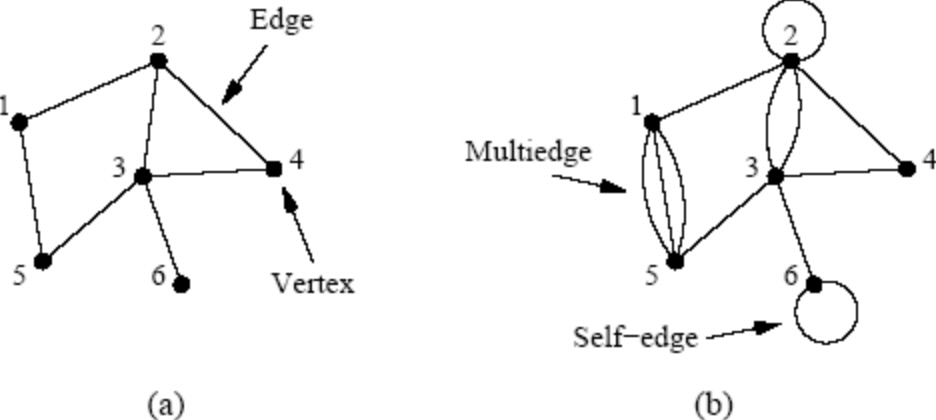
\includegraphics[width=0.5\linewidth]{Image.jpeg}
    \caption{Social network representation of gamer adoption: Nodes depict individual gamers and Edges represent peer influence. The imitation term in the Bass diffusion model is hence visualized. \cite{10.1093/acprof:oso/9780199206650.003.0006}.}
    \label{fig:GraphNodeFigure}
\end{figure}

\subsection{Compartmental Epidemics Model (Optional)}
If time permits, examining compartmental modelling focuses on population shifts between different groups within the population. Based on the Susceptible, Infectious, and Recovered individuals (SIR) model \cite{Hethcote2000Mathematics}, the population is divided into compartments of Potential Gamers, $S$; Active Gamers, $I$, and Retired/Past Gamers, $R$, each with their own growth rates:

\begin{equation}
\frac{dS}{dt} = -\beta S I, 
\qquad \frac{dI}{dt} = \beta S I - \gamma I, 
\qquad \frac{dR}{dt} = \gamma I
\end{equation}

\noindent Said equations are useful in studying churn rates, ``the rate at which customers stop doing business with an entity" \cite{INVESTOPEDIA2025CHURN}. This allows investigation of retired players returning to a game after new technologies arise.

\section{Timeline (Weekly Milestones)}

\begin{enumerate} [nosep]
    \item \textbf{Week of Oct. 5:} Review literature on adoption models; finalize metrics and collect data.
    \item \textbf{Week of Oct. 12:} Define core logistic--Bass hybrid model.
    \item \textbf{Week of Oct. 19:} Incorporate affordability and technological factors into the model.
    \item \textbf{Week of Oct. 26:} Implement computational simulations in Python.
    \item \textbf{Week of Nov. 2:} Analyze predictions and perform scenario testing (e.g., with/without VR).
    \item \textbf{Week of Nov. 9:} Organize results, integrate graphs/visuals, refine equations.
    \item \textbf{Week of Nov. 16:} Finalize report, verify the reproducibility of the code.
    \item \textbf{Week of Nov. 23:} Extra time reserved for contingencies and polishing.
\end{enumerate}



\section{Expected Outcomes}
Our group plans to deliver the following: 
\begin{itemize} [nosep]
    \item A validated and verified logistic–Bass hybrid model estimating the PC gamer population over time.
    \item Estimation of parameters from historical gamer adoption data.
    \item Case studies of disruptive technologies (VR, cloud gaming) on future growth.
    \item Graphical and computational products (e.g., simulations and sensitivity analysis).
    \item Discussion of model limitations and potential improvements (e.g., compartmental churn model and non-linear network effects).

\end{itemize}


\bibliographystyle{plain} % Or abbrv, unsrt, etc.
\bibliography{ref}
\end{document}